\documentclass[compress,handout,10pt]{beamer}

\newlength{\wideitemsep}
\setlength{\wideitemsep}{\itemsep}
\addtolength{\wideitemsep}{100pt}
\let\olditem\item
\renewcommand{\item}{\setlength{\itemsep}{0.5\baselineskip}\olditem}

\usetheme{AnnArbor}
\usecolortheme{crane}
\usefonttheme[onlymath]{serif}

\usepackage{float}
\floatstyle{boxed}
\usepackage{colortbl}
\usepackage{mathpazo}
\usepackage{graphicx}
\usepackage{movie15}
\usepackage{bm}
\usepackage{verbatim}
\usepackage{comment}
\usepackage{caption}
\usepackage{subcaption}
\captionsetup[subfigure]{labelformat=empty}
\captionsetup[figure]{labelformat=empty}

\newcommand{\mygreen}{\color{green!50!black}}
\newcommand{\myblue}{\color{blue}}
\newcommand{\myred}{\color{red}}
\newcommand{\mycolor}{\color{red}{c}\color{blue}{o}\color{green}{l}\color{orange}{o}\color{cyan}{r}}
\newcommand{\mysize}{\scriptsize{s}\small{i}\normalsize{z}\Large{e}}
\newcommand{\myshape}{\textcircled{s}\textit{h}\texttt{a}\textsf{p}\textsc{e}}

\xdefinecolor{titlecolor}{rgb}{.855,.647,.125}
\setbeamercolor{frametitle}{fg=titlecolor}
\setbeamerfont{frametitle}{series=\bfseries}
\setbeamercolor{normal text in math text}{parent=math text}

\setbeamertemplate{navigation symbols}{} %gets rid of navigation symbols
\setbeamertemplate{footline}[frame number]
\beamertemplateshadingbackground{blue!5}{yellow!10}

\title{{\color{blue} \LARGE Logistics of Constructing a Washington D.C.-Baltimore Rapid Transit Line\newline} }

\subtitle{{\large Washington Metropolitan Area Transit Authority \newline \large Maryland Transit Administration} }

\author{ 
%    \vspace{5pt}
    {\bf{Participant:}} \\ 
Danni Tang \\ 
    \vspace{5pt}
} 
\institute{Johs Hopkins University}

\date{\mygreen Last Complied on \today} 

\begin{document}

\begin{frame}[plain]
    \titlepage
\end{frame}

\begin{frame}
    \frametitle{Table of Contents}
    \tableofcontents
\end{frame}

\section{Sponsors and Relevance}

\begin{frame}
    \frametitle{Sponsors}
    Washington Metropolitan Area Transit Authority (WMATA):
    \vspace{7pt}
             \begin{enumerate}
                 \item transportation agency created by the Library of Congress
		 \item operates in the District of Columbia, Maryland, and the Commonwealth of Virginia
                 \item rapid transit service (Metrorail)
                 \item bus services (Metrobus)
                 \item paratransit (MetroAccess)
                 \item currently contructing new lines in Virginia (Silver Line) and in Maryland surburbs of D.C. (Purple Line)
             \end{enumerate}
\end{frame}

\begin{frame}
    \frametitle{Sponsors (cont.)}
    Maryland Transit System (MTA Maryland):
    \vspace{7pt}
             \begin{enumerate}
                 \item transportation agency operated by the state of Maryland
                 \item operates in the Baltimore-Washington Metropolitan area
                 \item numerous bus lines
                 \item Light Rail
                 \item Metro Subway
		 \item MARC train
             \end{enumerate}
\end{frame}

\begin{frame}
\frametitle{D.C. Metro Map}
\begin{figure}[h]
    \begin{center}
        \resizebox{0.6\textwidth}{!}{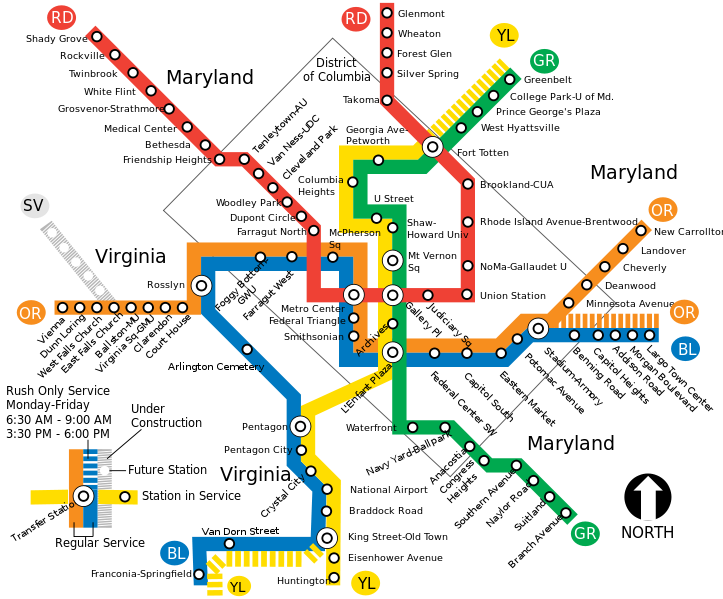
\includegraphics{WMATA_system_map.png}}
    \end{center}
    \caption{WMATA existing lines and stations, June 2012}
\end{figure}
\end{frame}

\begin{frame}
    \frametitle{Relevance}
    Problem area:
    \vspace{7pt}
     \begin{itemize}
	\item D.C. and Baltimore have similar worker populations
\begin{table}[ht]
\caption{Workers Who Use Public Transportation}   % title of Table
\centering % used for centering table
\begin{tabular}{c c c} % centered columns (3 columns)
\hline\hline %inserts double horizontal lines
City & \# of workers & \# of cars, trucks, or vans \\ [0.5ex]
\hline  % inserts single horizontal line
Washington, D.C. & 293,532 & 127,494 \\% inserting body of the table
Baltimore & 269,917 & 186,961 \\ [1ex] % [1ex] adds vertical space
\hline %inserts single line
\end{tabular}
\label{table:workers} % is used to refer this table in the text
\end{table}
	\item 43\% of D.C. workers commute in cars, trucks, or vans
	\item 69\% of Baltimore workers commute in cars, trucks, or vans
	\item it is apparent that large populations of workers of both cities rely heavily on vehicles to commute
	\item a subway line between the two cities would greatly reduce traffic volume, jams, and accidents
	\item sponsors would find this model relevant
     \end{itemize}
\end{frame}

\section{Problem Statement}

\begin{frame}
    \frametitle{Problem Statement}
    \begin{itemize}
        \item WMATA has no plans to expand the Metrorail system to the city and suburbs surrounding Baltimore
	\item MTA Maryland's Metro Subway system only operates within city limits
	\item residents of Greater Washington-Baltimore Metropolitan area have limited access to public transportation to travel between the two cities
	\item current public transportation methods:
	\begin{itemize}
		\item AMTRAK fares too expensive for daily commute
		\item MARC operates rush hours on weekdays
	\end{itemize}
	\item both sponsors operate under two separate government agencies
	\item our task is to provide a model that can predict the operating capacity for a such a line based on published transportation statistics
    \end{itemize}
\end{frame}

\begin{frame}
    \frametitle{Deliverables: From Sponsor to Team}
    \begin{enumerate}
        \item most recent data and statistics from Maryland Department of Transportation by Oct 19, 2012
	\begin{itemize}
		\item contingency plan: if data not received by the assigned time, we will obtain data published on the Department of Transportation website
	\end{itemize}
	\item computing resources
	\item timely responses to inquiries
	\item small expenses relevant to work
    \end{enumerate}
\end{frame}

\begin{frame}
    \frametitle{Deliverables: From Team to Sponsor}
    \begin{enumerate}
        \item mathematical model of traffic flow at various hours of the day (morning, noon, evening)
	\item traffic flow will model highways I-495 and I-95
	\item analytical report on the results of traffic flow model to determine if a subway line is viable
	\item time permitting, design of the subway line
	\item R package with documentations and codes to reproduce test results
	\item technical report and presentation summarizing the work done
    \end{enumerate}
\end{frame}

\section{Approach}
\begin{frame}
    \frametitle{Gathering the Data}
     \begin{enumerate}
	\item contact statisticians through sponsors at Maryland Department of Transportation for the most recent data on highway mobility and traffic trends between D.C. and Baltimore
	\item receive data through email (if electronic)
	\item receive data through regular mail (if paper copies)
	\item determine of data is relevant/useable to traffic model
	\item contact statisticians in the event of needing additional data
     \end{enumerate}
\end{frame}

\begin{frame}
    \frametitle{Gathering the Data - Contingency Plan}
    In the event that we do not receive data from Maryland Department of Transportation by Oct 19, 2012:
     \begin{enumerate}
    \vspace{7pt}
	\item visit the Maryland Department of Transportation website at \texttt{http://sha.md.gov/index.aspx?PageId=682}
	\item download "2012 Maryland State Highway Mobility Report"
	\item browse through "Traffic Trends" section
	\item look for other relevant sources through Google, such as MARC and AMTRAK train statistics
     \end{enumerate}
\end{frame}

\section{Traffic Flow Models}
\begin{frame}
    \frametitle{M. Bando Model of Optimal Velocity}
     \begin{enumerate}
	\item assumptions:
		\begin{itemize}
			\item Newtonian law of acceleration
			\item a car will drive at maximum speed with enough distance from the car in front
			\item a car will maintain optimal velocity depending on distance from the car in front
		\end{itemize}
	\item governing equations:
	\[
	\frac{dx_i}{dt} = v_i
	\]
	\[
	\frac{dx_i}{dt} = a[V(x_{i+1} - x_i) - v_i]
	\]
	\[
	V(b) = tanh(b-2) + tanh(2)
	\]
	\item initially, cars are uniform; traffic jam occurs when the model becomes unstable
     \end{enumerate}
\end{frame}

\begin{frame}
    \frametitle{Payne-Whitham Model}
     \begin{enumerate}
	\item assumptions
	\begin{itemize}
		\item single lane, straight roads
		\item drivers behave predictably and obey all traffic laws
	\end{itemize}
	\item governing system of equations:
	\[
	\rho_t + (\rho*v_*(\rho))_x = 0 
	\]
	\[
	v_t + vv_x + \frac{{c_0}^2}{\rho}\rho_x = \frac{v_*(\rho) - v}{\tau}
	\]
	\item at low traffic density, traffic flow is nice and uniform
	\item at high traffic density, flow becomes unstable when perturbations grow; instabilities become traveling waves called jamitons
     \end{enumerate}
\end{frame}

\begin{frame}
    \frametitle{Implementation of Traffic Flow Models}
     \begin{enumerate}
	\item both models of traffic flow will be simulated in MATLAB
	\item models will incorporate parameters from transportation data and statistics, such as number of cars traveling at certain times of day, average speed of cars, etc
	\item after simulating and comparing the two models, we will determine one model to realistically represent the highway traffic flow between D.C. and Baltimore
	\item using the chosen traffic model, we will determine if a rapid transit line is viable
     \end{enumerate}
\end{frame}

\section{Results}

\begin{frame}
    \frametitle{Report and Presentation}
     \begin{enumerate}
	\item analytical report on the results of traffic flow model simulations, such as accuracy of the model, the effect of changing model parameters on the model, etc
	\item determine viability of building a rapid transit line
	\item compose an R package with documentation and codes to reproduce results
	\item prepare a final report (paper and beamer presentation)
     \end{enumerate}
\end{frame}

\begin{frame}
    \frametitle{Design of Subway Line (Time Permitting)}
     \begin{enumerate}
	\item based on results from traffic flow simulation, decide if a rapid transit line is viable based on parameters such as number of commuters, reduction in frequency of traffic jams and accidents, and financial feasibility
	\item research the cost and logistics of building a line
	\item set fare prices for all stops (include a flat price)
	\item determine the locations of subway stops (places of highest traffic volume)
	\item number of subway stops will depend on optimal distances between stops
	\item predict the operating capacity of the subway transit line between D.C. and Baltimore
     \end{enumerate}
\end{frame}

\section{Checking Deliverables}
\begin{frame}
    \frametitle{Deliverables: From Sponsor to Team}
    \begin{enumerate}
        \item most recent data and statistics from Maryland Department of Transportation by Oct 19, 2012
	\begin{itemize}
		\item contingency plan: if data not received by the assigned time, we will obtain data published on the Department of Transportation website
	\end{itemize}
	\item computing resources
	\item timely responses to inquiries
	\item small expenses relevant to work
    \end{enumerate}
\end{frame}

\begin{frame}
    \frametitle{Deliverables: From Team to Sponsor}
    \begin{enumerate}
        \item mathematical model of traffic flow at various hours of the day (morning, noon, evening)
	\item traffic flow will model highways I-495 and I-95
	\item analytical report on the results of traffic flow model to determine if a subway line is viable
	\item time permitting, design of the subway line
	\item R package with documentations and codes to reproduce test results
	\item technical report and presentation summarizing the work done
    \end{enumerate}
\end{frame}

\section{Remaining Work and Future}
\begin{frame}
    \frametitle{Remaining Work}
  Since work has not begun on the project, we will need to initialize the project as soon as sponsors can provide the deliverables, or activate the contingency plan if they cannot.
  \vspace{7pt}
	\begin{itemize}
	\item wait for sponsors to send us data by Oct 19; if deadline not met, activate contingency plan
	\item determine which traffic flow model to use
	\item write MATLAB code of chosen traffic flow model, implement appropriate initial conditions from transportation data, and plot relevant graphs
	\item compose analytical report on results of traffic flow model and R package
	\item time permitting, design a subway line based on model
	\item presentation of completed work
	\end{itemize}
\end{frame}

\begin{frame}
    \frametitle{Future Research}
	\begin{itemize}
	\item look into other traffic flow models
	\item implement more factors other than highway mobility for a more realistic model
	\item look into MARC and AMTRAK statistics for a different model, since we did not account for the D.C.-Baltimore commuters who take these trains
	\item if subway design not completed due to limited time, design the line based on all models considered above
	\end{itemize}
\end{frame}

\begin{frame}[allowframebreaks]{Bibliography}
\frametitle{References}
\bibliographystyle{plain}
\nocite{*}
\bibliography{biblio}
\end{frame}
\end{document}
